\documentclass{article}
\usepackage[letterpaper]{geometry}
\geometry{verbose,tmargin=1in,bmargin=1in,lmargin=1in,rmargin=1in}

\usepackage[utf8]{inputenc}
\usepackage{amsmath}
\usepackage{listings}
\usepackage{graphicx}
\usepackage{enumitem}
\usepackage{amssymb}
\usepackage{tabularx}
\usepackage{hyperref}
\usepackage{caption}
\usepackage{float}
\usepackage[section]{placeins}

\title{CIS 419/519: Homework 5}
\author{Jiatong Sun}
\date{03/13/2020}

\begin{document}
    \maketitle
    \noindent
    Although the solutions are entirely my own, I consulted with the following people and sources while working on this homework: $Yuchen Sun$, $Junfan Pan$\\
    https://stackoverflow.com/questions/50994504/how-to-put-figure-between-items-on-enumerate-list
    
    \section{Logical Functions with Neural Nets}
        \begin{enumerate}[label=\alph*.]
            \item % a
				\begin{minipage}[t]{\linewidth}
                	\captionsetup{type=figure}
                	\centering
                	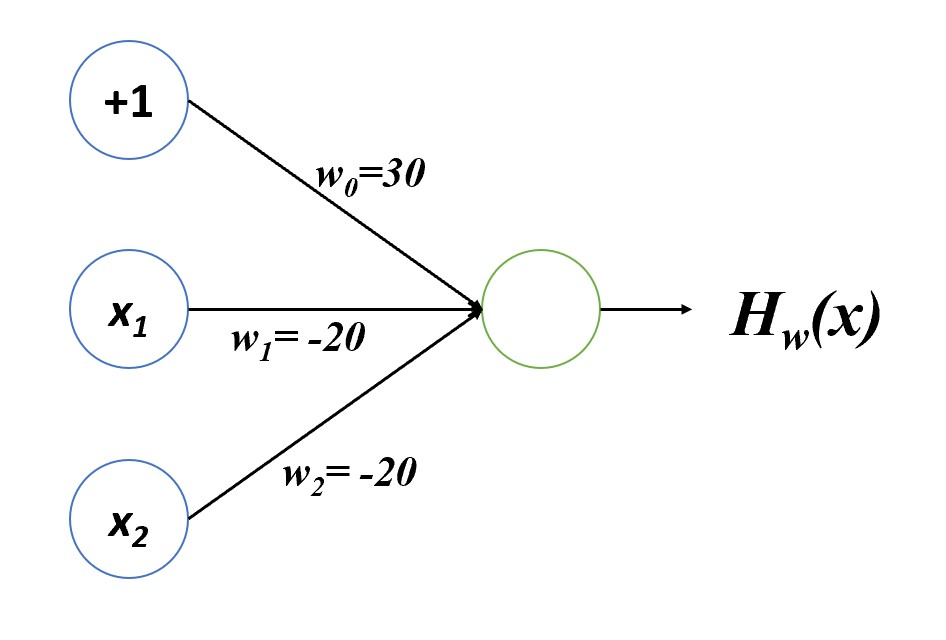
\includegraphics[width=0.6\linewidth]
                					{images/Q1a.jpg}
                	\caption{NAND}      
        		\end{minipage} 
        		
        		
        		\begin{table}[h]
        			\centering
					\begin{tabularx}{0.8\textwidth} { 
 						| >{\centering\arraybackslash}X 
  						| >{\centering\arraybackslash}X 
   						| >{\centering\arraybackslash}X | }
   						\hline
   						\multicolumn{3}{|c|}
   						{\textbf{Truth Table}}\\
 						\hline
 					 	$x_1$ & $x_2$ & $H(x)$ \\
 						\hline
 						0 & 0 & $\sigma(30)=1$\\
 						\hline
 						0 & 1 & $\sigma(10)=1$\\
 						\hline
 						1 & 0 & $\sigma(10)=1$\\
 						\hline
 						1 & 1 & $\sigma(-10)=0$\\
						\hline
					\end{tabularx} 
					\caption{NAND}
					\label{tab:1}
				\end{table}	        		           
            
            \item % b
            	\begin{minipage}[t]{\linewidth}
                	\captionsetup{type=figure}
                	\centering
                	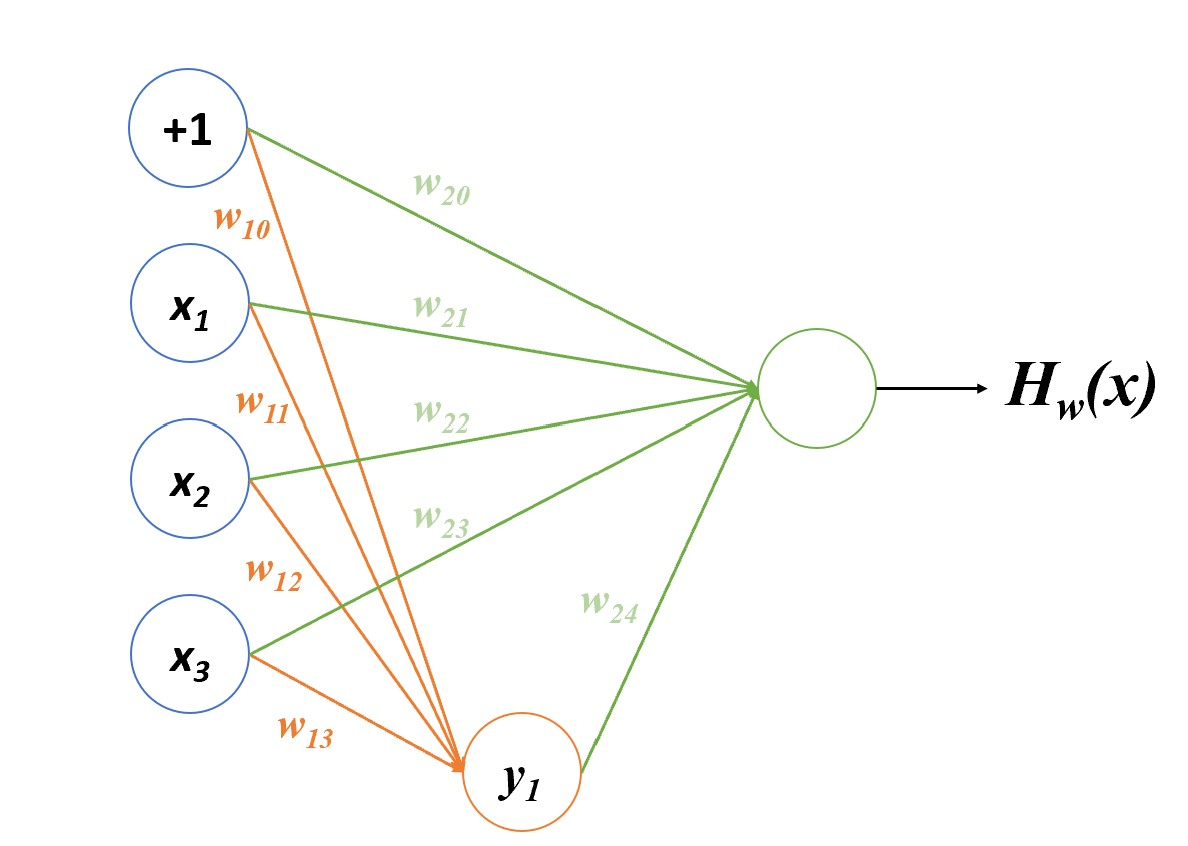
\includegraphics[width=0.6\linewidth]
                					{images/Q1b.jpg}
                	\caption{NAND}      
        		\end{minipage} 
        		
        		
        		\begin{table}[h]
        			\centering
					\begin{tabularx}{0.8\textwidth} { 
 						| >{\centering\arraybackslash}X 
  						| >{\centering\arraybackslash}X 
  						| >{\centering\arraybackslash}X 
  						| >{\centering\arraybackslash}X
  						| >{\centering\arraybackslash}X
  						| >{\centering\arraybackslash}X
  						| >{\centering\arraybackslash}X
  						| >{\centering\arraybackslash}X
   						| >{\centering\arraybackslash}X | }
   						\hline
   						\multicolumn{9}{|c|}
   						{\textbf{Truth Table}}\\
 						\hline
 					 	$w_{10}$ & $w_{11}$ & $w_{12}$ & $w_{13}$ &
 					 	$w_{20}$ & $w_{21}$ & $w_{22}$ & $w_{23}$ & 
 					 	$w_{24}$ \\
 						\hline
 						-30 & 20 & 20 & 20 & -10 & 20 & 20 & 20 & -40\\
 						\hline
					\end{tabularx} 
					\caption{Weight table}
					\label{tab:2}
				\end{table}	
        		
        		
        		\begin{table}[h]
        			\centering
					\begin{tabularx}{0.8\textwidth} { 
 						| >{\centering\arraybackslash}X 
  						| >{\centering\arraybackslash}X 
  						| >{\centering\arraybackslash}X 
  						| >{\centering\arraybackslash}X
   						| >{\centering\arraybackslash}X | }
   						\hline
   						\multicolumn{5}{|c|}
   						{\textbf{Truth Table}}\\
 						\hline
 					 	$x_1$ & $x_2$ & $x_3$ & $y_1$ & $H(x)$ \\
 						\hline
 						0 & 0 & 0 & $\sigma(-30)=0$ & $\sigma(-10)=0$\\
 						\hline
 						0 & 0 & 1 & $\sigma(-10)=0$ & $\sigma(10)=1$\\
 						\hline
 						0 & 1 & 0 & $\sigma(-10)=0$ & $\sigma(10)=1$\\
 						\hline
 						0 & 1 & 1 & $\sigma(-10)=0$ & $\sigma(10)=1$\\
 						\hline
 						1 & 0 & 0 & $\sigma(10)=1$ & $\sigma(-10)=0$\\
 						\hline
 						1 & 0 & 1 & $\sigma(10)=1$ & $\sigma(-10)=0$\\
 						\hline
 						1 & 1 & 0 & $\sigma(10)=1$ & $\sigma(-10)=0$\\
 						\hline
 						1 & 1 & 1 & $\sigma(30)=1$ & $\sigma(10)=1$\\
						\hline
					\end{tabularx} 
					\caption{Parity}
					\label{tab:3}
				\end{table}	  
            
        \end{enumerate}
        
    \section{Calculating Backprop by Hand}
    	Since the hidden layer uses a sign function and the output layer uses a sigmoid function, the output can be expressed as follows:
    	$$a_2(\boldsymbol{X})=
    	Sigmoid(b_2(\boldsymbol{X}))=
    	\dfrac{1}{1+e^{-b_2(\boldsymbol{X})}}=
    	\dfrac{1}{1+e^{-\boldsymbol{W^2}a_1(\boldsymbol{X})}}=
    	\dfrac{1}{1+e^{-\boldsymbol{W^2}\cdot Sign(\boldsymbol{W^1}\boldsymbol{X})}}$$
    	where
    	$$a_1(\boldsymbol{X})=
    	Sign(b_1(\boldsymbol{X}))=
    	Sign(\boldsymbol{W^1}\boldsymbol{X})=
    	Sign(\begin{bmatrix}0.1 & 0.2\\-0.4 & 0.3\end{bmatrix} \begin{bmatrix}5\\4\end{bmatrix})=
    	Sign(\begin{bmatrix}1.3\\-0.8\end{bmatrix})=
    	\begin{bmatrix}1\\-1\end{bmatrix}$$
    	and
    	$$a_2(\boldsymbol{X})=
    	\dfrac{1}{1+e^{-\boldsymbol{W^2}a_1(\boldsymbol{X})}}=
    	\dfrac{1}{1+e^{-\begin{bmatrix}0.1&0.2\end{bmatrix}\begin{bmatrix}1\\-1\end{bmatrix}}}=
    	\dfrac{1}{1+e^{0.1}}=0.475$$
    	To calculate the output gradient with respect to each of the weights, we can use the chain rule and thus, we know that
    	$$\dfrac{da_2(\boldsymbol{X})}{d\boldsymbol{W^2}}=
    	\dfrac{da_2(\boldsymbol{X})}{db_2(\boldsymbol{X})}\dfrac{db_2(\boldsymbol{X})}{d\boldsymbol{W^2}}=
    	[a_2(\boldsymbol{X})(1-a_2(\boldsymbol{X}))]\cdot a_1(\boldsymbol{X})=0.475\cdot(1-0.475)\cdot\begin{bmatrix}1\\-1\end{bmatrix}=\begin{bmatrix}0.249\\-0.249\end{bmatrix}$$
    	$$\dfrac{da_2(\boldsymbol{X})}{d\boldsymbol{W^1}}=
    	\dfrac{da_2(\boldsymbol{X})}{db_2(\boldsymbol{X})}\dfrac{db_2(\boldsymbol{X})}{da_1(\boldsymbol{X})}\dfrac{da_1(\boldsymbol{X})}{db_1(\boldsymbol{X})}\dfrac{db_1(\boldsymbol{X})}{d\boldsymbol{W^1}}=
    	0.249\cdot\boldsymbol{W^2}\cdot\begin{bmatrix}0\\1\end{bmatrix}\cdot\boldsymbol{W^1}=0.249\cdot\begin{bmatrix}0.1&0.2\end{bmatrix}\cdot\begin{bmatrix}0\\1\end{bmatrix}\cdot\begin{bmatrix}0.1 & 0.2\\-0.4 & 0.3\end{bmatrix}=\begin{bmatrix}0.005 & 0.01\\-0.02 & 0.015\end{bmatrix}$$
    	$$$$
			
        
    \section{Neural Nets in SuperTuxKart}
       
\end{document}